% Use the "article" document class with 12pt font and A4 paper size
\documentclass[12pt,a4paper]{article}
\usepackage{amsmath}
\usepackage[utf8]{inputenc}
\usepackage{caption}
\usepackage{array}
\usepackage{booktabs}
\usepackage{float}
\usepackage{xcolor}
% Set the document language to English
\usepackage[english]{babel}

% For URLs
\usepackage[hidelinks]{hyperref}
\usepackage{subcaption}

% For using circuits
\usepackage{circuitikz}

% Allow image inclusion
\usepackage{graphicx}
\usepackage{titlesec}
\titleformat{\section}[block]{\normalfont\Large\bfseries}{\thesection}{0.5cm}{}
\renewcommand{\contentsname}{\LARGE Contents}

% Page margins
\usepackage[top=1in, bottom=1in, left=1in, right=1in]{geometry}

% Diagram packages
\usepackage{tikz}
\usetikzlibrary{positioning, arrows.meta, shapes.geometric}

% Define a custom horizontal rule
\newcommand{\HRule}{\rule{\linewidth}{0.5mm}}

\begin{document}

\begin{titlepage}
\begin{center}


\includegraphics[width=0.75\textwidth]{IITD_AD_Logo_1709620040.png}~\\[1cm]

\HRule \\[0.4cm]
{ \LARGE 
  \textbf{ACOP290 C Project Report}\\[0.4cm]
  \emph{Spreadsheet program}\\[0.4cm]
}
\HRule \\[1.5cm]

{ \large
  Authors: Abhiramachandra Vemparala, Mohammad Taqi Ahsan \\[0.4cm]
  Date Submitted: 26\textsuperscript{th} April 2026 \\[0.5cm]
  Instructor: Prof. Kumar Madhukar\\[0.5cm]
  Academic Year: 2025--26\\[0.5cm]
  Source Code (GitHub): \href{https://github.com/abhivemparala/C-Project.git}{\textcolor{red}{Link}}\\[0.4cm]
}

\vfill

\textbf{\large Design Practices\\[0.4cm]Indian Institute of Technology Delhi - Abu Dhabi}\\[0.4cm]

\end{center}
\end{titlepage}

\tableofcontents
\newpage

\section{Overview}

This project implements a spreadsheet engine in C. The program provides a command-line interface with a visible 10$\times$10 grid, support for cell assignment, arithmetic expressions, range-based functions, scrolling commands, and dependency-driven recalculation.\\[0.1cm]

The implementation is divided into three main source files: \texttt{main.c}, \texttt{sheet.c}, and \texttt{parser.c}. This modular structure separates user interaction, spreadsheet data management, and expression parsing, making the code easier to maintain and debug.

\section{Architecture and Design}

\subsection{File Responsibilities}

\textbf{\texttt{main.c}}
\begin{itemize}
    \item Handles command-line argument validation and program startup.
    \item Maintains the main REPL (read-eval-print loop).
    \item Prints the spreadsheet view and processes commands such as \texttt{q}, \texttt{scroll\_to}, \texttt{disable\_output}, and \texttt{enable\_output}.
    \item Delegates formula parsing and execution to \texttt{parser.c}.
\end{itemize}

\noindent\textbf{\texttt{sheet.c}}
\begin{itemize}
    \item Implements the core spreadsheet data model and view state.
    \item Stores cells in a flattened array for constant-time access.
    \item Maintains the dependency graph used for recalculation.
    \item Implements scrolling and propagation of cell updates.
\end{itemize}

\noindent\textbf{\texttt{parser.c}}
\begin{itemize}
    \item Parses cell names, numeric values, formulas, functions, and binary expressions.
    \item Identifies dependencies created by cell references and ranges.
    \item Detects invalid syntax, invalid cells, invalid ranges, and circular dependencies.
    \item Evaluates expressions and reports runtime errors such as division by zero.
\end{itemize}

\subsection{Core Data Structures}

The spreadsheet state is represented through a \texttt{Sheet} structure containing:
\begin{itemize}
    \item \texttt{rows, cols}: dimensions of the full sheet.
    \item \texttt{view\_row, view\_col}: coordinates of the top-left visible cell.
    \item \texttt{cells}: a flattened array of all spreadsheet cells.
    \item \texttt{deps}: a dynamic array of dependency edges between cells.
\end{itemize}

\noindent Each \texttt{Cell} stores:
\begin{itemize}
    \item its type, such as value or error,
    \item the evaluated integer result,
    \item the original formula text if the cell was assigned a formula,
    \item an error flag for propagation,
    \item and a flag indicating whether the cell is formula-driven.
\end{itemize}

The Dependency graph uses a dynamic edge where the dependencies are represented using directed edges. If cell \texttt{B2} depends on \texttt{A1}, then an edge is created from \texttt{A1} to \texttt{B2}. This makes it possible to identify which cells must be recalculated when a source cell changes.\\[0.1cm]

Figure~\ref{fig:architecture} shows the overall software structure of the spreadsheet program. It illustrates how user commands are processed through the main control loop, parsed into expressions or commands, applied to the spreadsheet data model, and then propagated through the dependency graph for recalculation.

\begin{figure}[H]
\centering
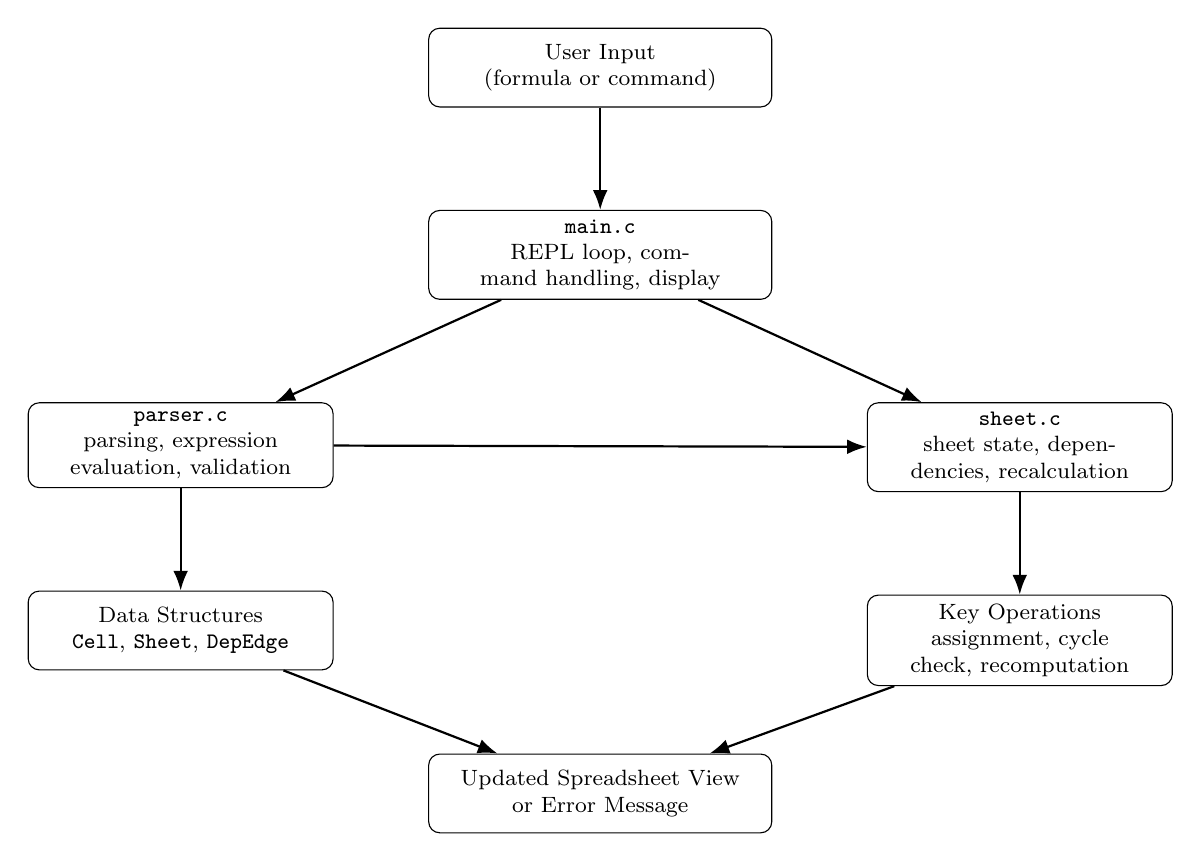
\begin{tikzpicture}[
    node distance=1.3cm and 1.2cm,
    box/.style={
        draw,
        rounded corners,
        align=center,
        text width=0.34\textwidth,
        minimum height=1cm,
        font=\footnotesize
    },
    smallbox/.style={
        draw,
        rounded corners,
        align=center,
        text width=0.30\textwidth,
        minimum height=1cm,
        font=\footnotesize
    },
    arrow/.style={
        -{Latex[length=2.5mm]},
        thick
    }
]

% Top
\node[box] (user) {User Input\\(formula or command)};

% Main controller
\node[box, below=of user] (main) {\texttt{main.c}\\REPL loop, command handling, display};

% Two middle modules
\node[smallbox, below left=of main] (parser) {\texttt{parser.c}\\parsing, expression evaluation, validation};
\node[smallbox, below right=of main] (sheet) {\texttt{sheet.c}\\sheet state, dependencies, recalculation};

% Data + operations
\node[smallbox, below=of parser] (data) {Data Structures\\\texttt{Cell}, \texttt{Sheet}, \texttt{DepEdge}};
\node[smallbox, below=of sheet] (ops) {Key Operations\\assignment, cycle check, recomputation};

% Output
\node[box, below=1.5cm of $(data)!0.5!(ops)$] (output) {Updated Spreadsheet View\\or Error Message};

% Arrows
\draw[arrow] (user) -- (main);
\draw[arrow] (main) -- (parser);
\draw[arrow] (main) -- (sheet);
\draw[arrow] (parser) -- (data);
\draw[arrow] (sheet) -- (ops);
\draw[arrow] (parser) -- (sheet);
\draw[arrow] (data) -- (output);
\draw[arrow] (ops) -- (output);

\end{tikzpicture}
\caption{Software structure of the spreadsheet program showing key files, data structures, and execution flow}
\label{fig:architecture}
\end{figure}

\section{Parsing and Evaluation}

The parser accepts formulas of the form \texttt{CELL = EXPR} and also handles commands such as \texttt{scroll\_to}. Supported expressions include:
\begin{itemize}
    \item integer constants, including negative numbers,
    \item cell references such as \texttt{A1},
    \item binary operations \texttt{+}, \texttt{-}, \texttt{*}, and \texttt{/},
    \item range-based functions such as \texttt{SUM}, \texttt{MIN}, \texttt{MAX}, \texttt{AVG}, and \texttt{STDEV},
    \item and ranges written in the form \texttt{A1:B3}.
\end{itemize}

Expression evaluation returns a structured result that explicitly records whether evaluation succeeded or failed. This avoids hidden behaviour and makes error handling more predictable. Runtime conditions such as invalid cells, division by zero, or malformed expressions are converted into spreadsheet errors that can also propagate to dependent cells.

\section{Dependency Graph and Recalculation}

Whenever a formula is assigned to a cell, its old dependencies are first removed. The parser then scans the formula again and rebuilds the dependency edges based on every referenced cell or range.\\[0.1cm]

To prevent invalid spreadsheet states, circular dependency detection is performed before finalizing the assignment. If assigning a formula would create a cycle, the assignment is rejected and the previous state is restored.\\[0.1cm]

When a cell is updated successfully, recalculation is performed only for cells affected by that change i.e. instead of recomputing the entire spreadsheet, the program traverses the dependency graph starting from the modified cell and reevaluates all dependent formulas. This approach improves efficiency and keeps updates localized.

\section{Error Handling and Edge Cases}

The spreadsheet explicitly handles a variety of invalid inputs and runtime issues:

\begin{itemize}
    \item \textbf{Invalid commands:} Input that does not match a recognized command or assignment is reported as an unrecognized command.
    \item \textbf{Invalid cell names:} Malformed references or out-of-range coordinates are rejected.
    \item \textbf{Invalid ranges:} Backward ranges such as \texttt{B2:A1} are treated as invalid.
    \item \textbf{Circular dependencies:} Assignments that introduce cycles are refused.
    \item \textbf{Division by zero:} Any expression involving division by zero marks the target cell as an error.
    \item \textbf{Error propagation:} If a formula depends on a cell already in an error state, the dependent formula also evaluates to an error.
\end{itemize}


\section{Test Suite Coverage}

The project includes a set of tests that run using the 'make test' command.

\subsection{Core Functionality Tests}

\begin{itemize}
    \item \texttt{test\_basic.c}: verifies startup behaviour, prompt rendering, and handling of invalid commands.
    \item \texttt{test\_arithmetic.c}: checks basic formula evaluation and arithmetic correctness.
    \item \texttt{test\_sum\_function.c}: validates summation across ranges.
    \item \texttt{test\_scroll\_to.c}: confirms correct scrolling and visible window updates.
\end{itemize}

\subsection{Robustness Tests}

\begin{itemize}
    \item \texttt{test\_recalc.c}: ensures dependent cells are updated correctly after source changes.
    \item \texttt{test\_div\_zero\_propagation.c}: confirms division-by-zero errors propagate as expected.
    \item \texttt{test\_invalid\_range.c}: tests malformed and backward ranges.
    \item \texttt{test\_invalid\_cell\_range.c}: checks handling of out-of-bounds range references.
\end{itemize}


\section{Challenges and Design Decisions}

One of the main challenges in this project was combining a simple expression evaluator with reliable dependency tracking. Formula evaluation had to remain straightforward while still supporting recalculation and error propagation across referenced cells.\\[0.1cm]

A significant design choice was storing cells in a flattened one-dimensional array instead of a traditional two-dimensional allocation. This simplifies memory management and indexing.\\[0.1cm]

Another important decision was representing dependencies as a dynamic edge list. Although more advanced graph structures are possible, an edge list was sufficient for cycle detection, dependency tracking, and recalculation while keeping the implementation relatively simple.

\end{document}